%%%%%%%%%%%%%%%%%%%%%%%%%%%%%%%%%%%%%%%%%%%%%%%%%%%%%%%%%%%%%%%%%%%%%%%%%%%%%%%%
% Copyright 2021 Louis Paternault --- http://ababsurdo.fr
%
% Publié sous licence Creative Commons Attribution-ShareAlike 4.0 International (CC BY-SA 4.0)
% http://creativecommons.org/licenses/by-sa/4.0/deed.fr
%%%%%%%%%%%%%%%%%%%%%%%%%%%%%%%%%%%%%%%%%%%%%%%%%%%%%%%%%%%%%%%%%%%%%%%%%%%%%%%%

% Pour compiler :
%$ lualatex $basename

\documentclass[12pt]{article}

\usepackage{2122-pablo}
\usepackage{2122-pablo-paternault}
\usepackage{2122-pablo-math}
\usepackage{2122-pablo-tikz}

\usepackage[
	includehead,
	a5paper,
	margin=1cm,
]{geometry}
\usepackage{2122-pablo-header}
\fancyhead[C]{\textsc{Ex. 4 p. 74 --- Correction}}

\begin{document}

\begin{exercice}[Exercice 4 page 74]~
\begin{enumerate}
\item Puisque Paul est ami avec Jeanne et Yassine, le sommet \enquote{Paul} est relié avec les deux sommets \enquote{Jeanne} et \enquote{Yassine}. Le dernier sommet est donc celui de \enquote{Nathan}. Remarquons que les deux sommets \enquote{Jeanne} et \enquote{Yassine} sont interhangeables.
\begin{center}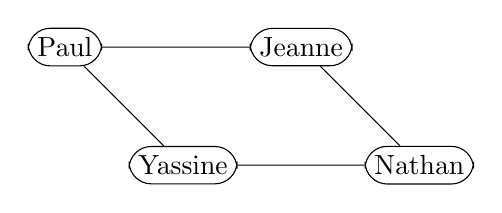
\begin{tikzpicture}[
	scale=1.5,
	sommet/.style={draw=black, rounded corners=8pt},
]
\node[sommet] (P) at (0, 0) {Paul};
\node[sommet] (J) at (2, 0) {Jeanne};
\node[sommet] (Y) at (1, -1) {Yassine};
\node[sommet] (N) at (3, -1) {Nathan};
\draw  (P) -- (J) -- (N) -- (Y) -- (P);
\end{tikzpicture}\end{center}
\item Calculons l'écartement de chacun des sommets.
Pour \enquote{Paul}, par exemple, le sommet le plus éloigné est \enquote{Nathan}, situé à une distance de 2 (il faut traverser au minimum deux arêtes pour l'atteindre). De même pour les autres sommets.
\begin{center}\begin{tabular}{r*{4}{c}}
\toprule
Sommet & Paul & Jeanne & Yassine & Nathan \\
\midrule
Écartement & 2 & 2 & 2 & 2\\
\bottomrule
\end{tabular}\end{center}
Calculons le diamètre, et --- même si ça n'était pas demandé --- le centre et le rayon.
\begin{itemize}
\item Le diamètre est le plus grand écartement, soit 2.
\item Le rayon est le plus petit écartement, soit 2 aussi.
\item Le centre est le sommet qui a le plus petit écartement, donc chacun des quatre sommets est un centre.
\end{itemize}
\end{enumerate}
\end{exercice}

\end{document}
